This is where we discuss the main results we've had.

\section{Estimating $c_{D}$ from Experiments}

\begin{itemize}
\item We try to find results for spheres and change them to account for the earlier drag crisis.
\item Take the function from \citet{Morrison2010} and change the coefficents to ``move'' the drag 
drop to lower values of $Re$.
\item This works fairly well but cannot capture all of the behaviour, as other work shows that
different balls should expect to see different drags \citet{Alam2011}.
\end{itemize}

\begin{figure}[h]
\centering
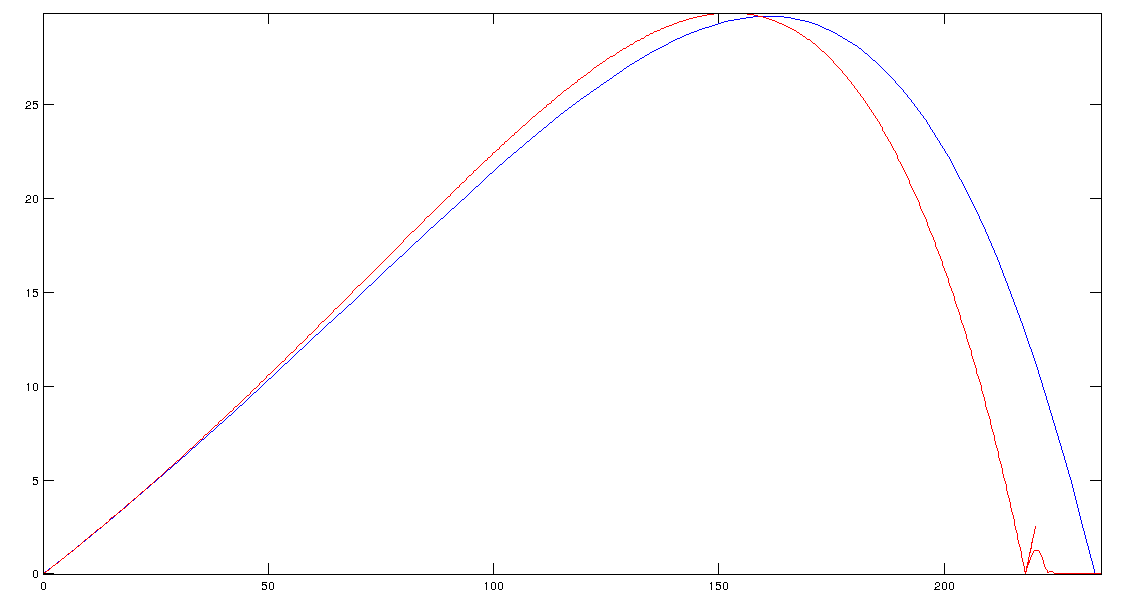
\includegraphics[scale=0.45]{../images/trajectory-older.png}
\caption[Model with $c_{D}$ dependent on $Re$.]{Using the modified Morrison form for $c_{D}$ results 
in a fairly accurate profile. Here red is the data and blue is the predictions of the model.}
\end{figure}

\begin{figure}[h]
\centering
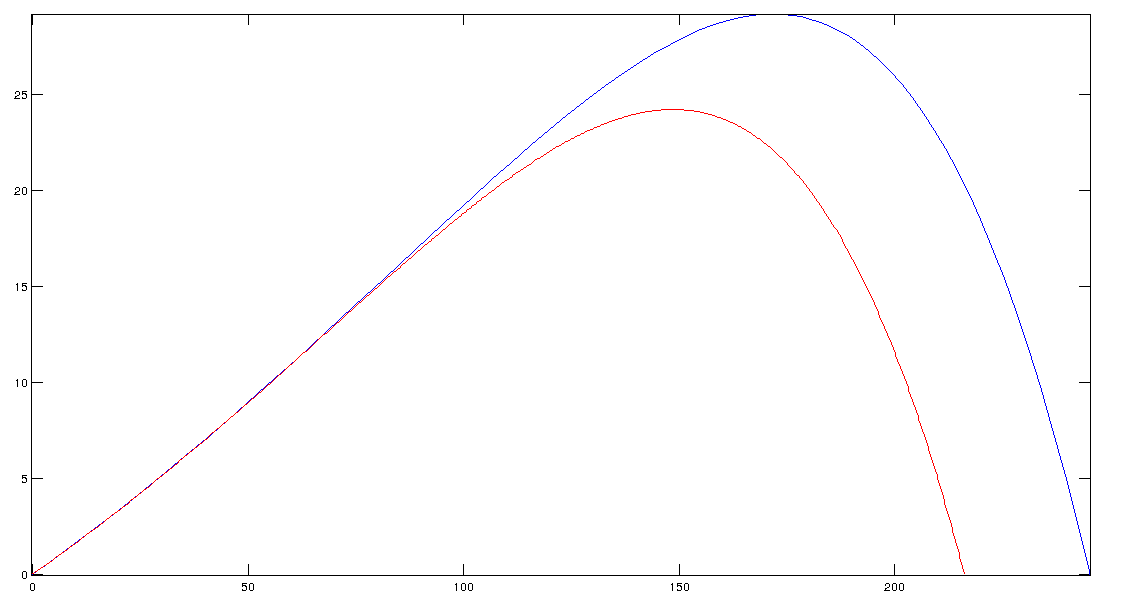
\includegraphics[scale=0.45]{../images/trajectory.png}
\caption[Second data set with Morrison drag.]{The Morrison drag form does not always produce accurate
results, however we do see good agreement at the start. Here red is the data and blue is the 
predictions of the model.}
\end{figure}

\section{Parameterising $c_{D}$ and $c_{L}$ by Non Dimensional Variables}

\begin{itemize}
\item We follow the idea from \citet{Lieberman2001}: form $c_{D}$ and $c_{L}$ from dimensionless
groupings and use the data to estimate the parameters in this model.
\item Use least squares to do this. See Appendix for discussion of what an inverse problem is, how
to use least squares to solve them, and what numerical techniques there are to do this.
\item Find that doing this is very hard: the problem is likely not well posed and finding a minimum
is difficult. Would benefit from a more through analysis of the least squares problem but unsure how
this would be done.
\item This inverse problem is a good way to move forwards with the problem in the future.
\end{itemize}

\section{$\tanh$ Matching}

\begin{itemize}
\item Take a hybrid approch between the two previous ideas: form a function which ``looks'' similar
to \citet{Morrison2010} and has the same behaviour, but is parameterised in such a way as to allow
us to use a least squares solver to estimate parameters.
\item For the drop, use a $\tanh$ function of the form
\[
c_{D} = a + b \tanh (-c(Re - d))
\]
where $a,b,c,d$ are constants which we can use least squreas to determine.
\item Match the $\tanh$ at the top with the $24/Re$ form we know from spheres and past the drop match
to the weakly linear form we see from the previous work.
\item Still trying to decide on results for this.
\end{itemize}